\documentclass{article}

\usepackage{amsmath}
\usepackage{booktabs}  % nice tables
\usepackage[margin=25mm]{geometry}
\usepackage[natbib=true,style=authoryear]{biblatex}
% NOTE : this file is automatically generated from Zotero, do not edit
% manually!
\addbibresource{references.bib}
\usepackage{siunitx}  % use for all units
\usepackage{subcaption}  % for subfigures
\usepackage[]{todonotes}  % use [disable] to hide notes

% NOTE : Use as \si{\kph} or \si{\mps}
\def\kph{\kilo\meter\per\hour}
\def\mps{\meter\per\second}

\title{Automatic Bicycle Balance Assistance Reduces Probability of Falling at
Low Speeds When Subjected to Handlebar Perturbations\\Version 2.dev}

\author{Marten T. Haitjema \and Leila Alizadehsaravi \and Jason K. Moore}

\begin{document}

\maketitle

\abstract{
  Uncontrolled bicycles are generally unstable at low speeds. We add an
  automatically controlled steering motor to a consumer electric bicycle that
  has a stabilizing effect down to about 3~\si{\kph}. We hypothesize that a
  stabilized bicycle will reduce the probability of falling. To test the
  motor's possible assistance during falls, we apply varying magnitude external
  handlebar perturbations to twenty-six participants who rode on a treadmill
  with the balance assist system activated and deactivated. The probability of
  recovering from a handlebar perturbation significantly increases when the
  balance assist is activated at a travel speed of 6~\si{\kph}. This positive
  effect is most prominent at and around the individual riders' perturbation
  resistance threshold. We conclude that use of a balance assist system in real
  world bicycling would reduce the number of falls that occur near riders'
  control authority limits.
}

\section{Introduction}
%
Single-actor bicycle crashes are associated with a surprisingly large
percentage of reported serious injuries~\citep{Wegman2024}. At low speeds, from
start up to typical cruising speeds, bicycles are not self-stable and can be
challenging for the rider to balance. Low speed crashes may be reduced if the
bicycle was self-stable at these speeds by relieving the rider of some of their
necessary control activity. Bicycles can be mechanically modified to lower the
speeds at which they are self-stable~\citep{Astrom2005} and since the 1980s it
has been known that applying a motor actuated steering torque proportional to
the vehicle's roll angular rate~\footnote{Roll angular rate is defined herein
as per the SAE J670 vehicle standards.} can stabilize a single-track vehicle
down to very low speeds. If automatic control of steering can stabilize a
bicycle, it may reduce the control required from the rider to successfully
manage balancing tasks much like the natural high speed self-stability already
does. We have developed a balance-assisting bicycle,
Figure~\ref{fig:balance-assist-bicycle}, based on these principles and
hypothesize that it helps the rider in situations in which they are likely to
fall.
%
\begin{figure}
  \centering
  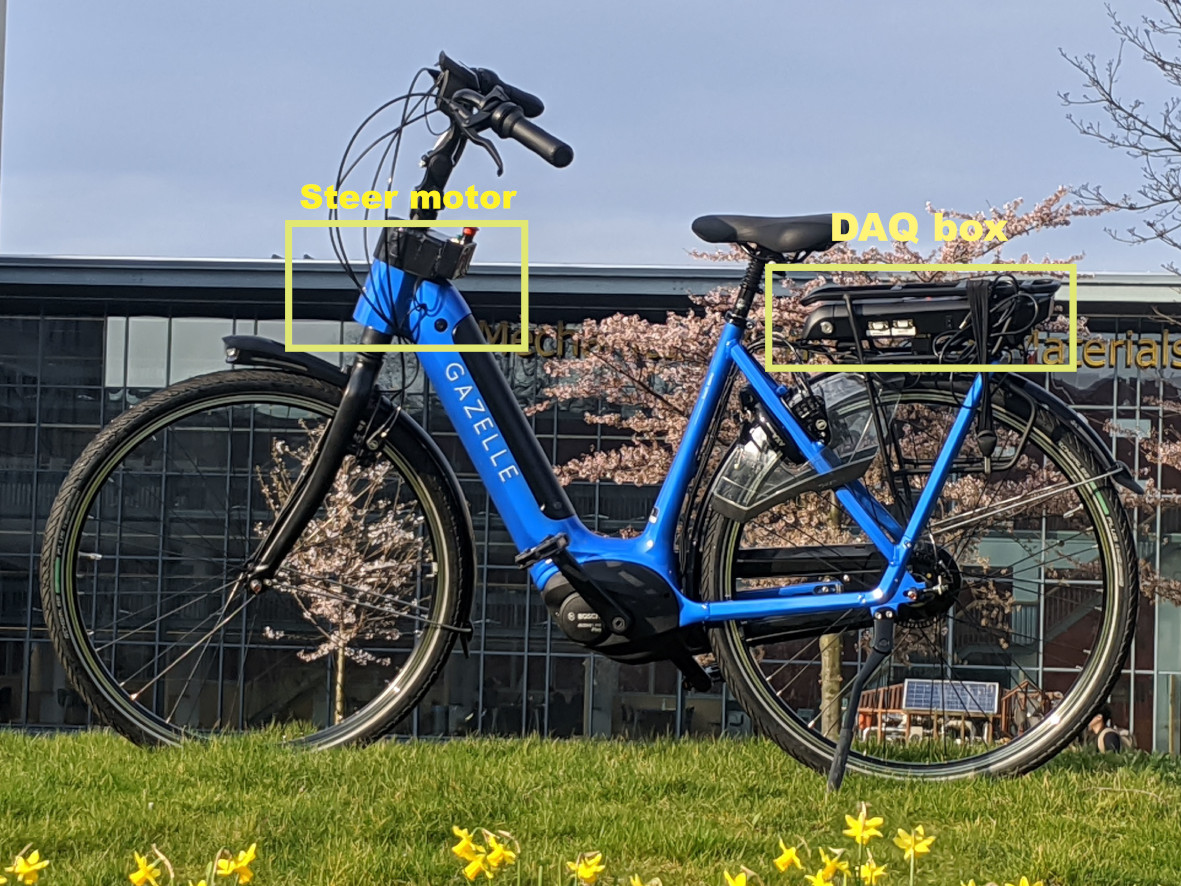
\includegraphics[width=80mm]{figures/balance-assist-bicycle.jpg}
  \caption{Balance assist bicycle prototype with electric motor in the steering
    column and data acquisition and control electronics mounted in the rear
    rack.}
  \label{fig:balance-assist-bicycle}
\end{figure}

Riders fall when their control authority is not able to maintain a stable
vehicle state. There are many real world scenarios that can put the vehicle
into an uncontrollable state. External forces applied to the vehicle or rider
are one such scenario type and natural examples include wind gusts, handlebars
colliding with a neighbor's, a bag swinging from the handlebar, or simply
hitting a bump in the road. To assess our balance assisting bicycle, we subject
the rider to perturbations at the handlebar, which can relatively easily cause
a rider to fall.

In this paper, we test whether a steer motor controlled bicycle, that is stable
in a large low speed range, is beneficial in helping to prevent the rider from
falling. We test this by applying varying magnitude mechanical perturbations to
the handlebars while the rider is cycling on a treadmill. We assess the
difference in the rider's probability of falling with the balance assist system
on and off.

\subsection{Technical Background}
%
During the early years of developments in automatic control,
\citep{Whipple1899} not only derived the correct equations of motion of the
bicycle \citep{Meijaard2007} but realized and showed that roll motion feedback
can stabilize a bicycle. Much later, attempts at automatic roll stabilization
of single-track vehicles began in earnest after predictive motorcycle models
were developed and refined throughout the 1970s. \Citet{vanZytveld1975} was
influenced by Whipple's work and seems to be the first to attempt to
robotically stabilize a small motorbike with a controlled inverted pendulum
that mimicked rider lean, but he was not successful in demonstrating what his
theoretic control model correctly predicted. In his model, he recognized that
feedback of the vehicle roll angle and angular rate was essential to stabilize
the vehicle. It was not until the early 1980s that \cite{Nagai1983}
successfully demonstrated balancing a robotic bicycle on a treadmill with both
steering control and a laterally moving mass. \citet{Ruijs1986} followed this
breakthrough by demonstrating an automatically balanced motorcycle and they did
so solely with a steering motor. Ruijs and Pacejka clearly showed that steer
torque driven by roll angle feedback stabilizes the capsize mode, by roll
angular rate feedback stabilizes the weave mode, and by steer angular rate
feedback stabilizes the wobble mode.~\footnote{These motorcycle (and bicycle)
eigenmodes are defined in \citep{Sharp1971}.} They also showed how the control
gains must change with respect to vehicle speed for favorable control across
all speeds. This roll motion feedback enables the simplest controller that can
stabilize a single-track vehicle above a minimum speed when one is not
concerned with wobble instabilities. But Ruijs and Pacejka's work was not
particularly concerned with low speed stability and their vehicle was fully
automatic, i.e no human rider was involved.

Many more automatically balanced single-track vehicles have been demonstrated
over the last 40 years, but none have demonstrated that increasing low speed
stability can assist in human balancing and what effect it may have towards
single-actor falls. Most of these robotic bicycle and motorcycle designers did
not intend for a human rider to also control the stabilized vehicle.
Nevertheless, an automatically stabilized bicycle can be controlled by a human
rider if the motor controlled steer torque and the rider applied steer torque
act on the steer in parallel. The effect of this automatic control gives the
ability to effectively change the human-controlled plant dynamics, up to some
limits. In our prior study~\citep{Alizadehsaravi2023}, we demonstrate reduced
motion during distractions due to the balance assist system but
\citet{Hanakam2023} recently showed rider dissatisfaction with the
stabilization of a similar vehicle so the possible benefits are not
definitively established.

The design of a balance assist system relies on the linear Carvallo-Whipple
bicycle model~\citep{Carvallo1899,Whipple1899} which is the simplest bicycle
model that exhibits non-minimum phase behavior and self-stability. The bicycle
model is well suited for showing the effect of a roll motion feedback driven
steer motor on the dynamics. This model is equivalently valid for on-road or
treadmill riding~\citep{Kooijman2009a}, which have the same fundamental
dynamics. The linear version of this model can be described by the fourth order
state space equations:
%
\begin{align}
  \dot{\vec{x}} = \mathbf{A} \vec{x} +
  \mathbf{B}
  \vec{u}
  \textrm{ where }
  \vec{x} = \begin{bmatrix} \phi \\ \dot{\phi} \\ \delta \\ \dot{\delta} \end{bmatrix}
  \textrm{ and }
  \vec{u} = \begin{bmatrix} T_{\phi} \\ T_{\delta} \end{bmatrix}
  \textrm{.}
\end{align}
%
The states \(\vec{x}\) are the roll angle \(\phi\) and steer angle \(\delta\)
along with their time derivatives and the inputs \(\vec{u}\) are roll torque
\(T_\phi\) and steer torque \(T_\delta\). The state matrix \(\mathbf{A}\) is a
function of the equilibrium forward speed \(v\). It and the input matrix
\(\mathbf{B}\) are otherwise populated with expressions that are functions of
the geometric and inertial parameters of the nonholonomic multibody system made
up of four rigid bodies: two wheels, front frame, and rear frame.

If the steer torque is the sum of the (h)uman applied torque and the (m)otor
applied torque \(T_\delta = T_\delta^\textrm{h} + T_\delta^\textrm{m}\),
\(\mathbf{B} = \begin{bmatrix} \vec{B}_\phi \quad \vec{B}_\delta
\end{bmatrix}\), and the motor torque is a proportional feedback controller
\(T_\delta^\textrm{m} = -k_{\dot{\phi}} \dot{\phi}\) then the human-controlled
plant takes the form:
%
\begin{align}
  \dot{\vec{x}} = \left(\mathbf{A} -
  \vec{B}_\delta
  \left[0 \quad k_{\dot{\phi}} \quad 0 \quad 0\right]
\right)
  \vec{x} + \mathbf{B} \begin{bmatrix} T_{\phi} \\ T_\delta^\textrm{h} \end{bmatrix}
\end{align}

The state matrix \(\mathbf{A}\) being a function of the equilibrium speed \(v\)
means the control gain \(k_{\dot{\phi}}\) can be selected such that the
eigenvalues of \(\left(\mathbf{A} - \vec{B}_\delta\left[0 \quad k_{\dot{\phi}}
\quad 0 \quad 0\right] \right)\) have negative real parts for \(v_{min} < v <
v_\textrm{capsize}\) where \(v_{min}\) is the lowest stable speed given
\(k_{\dot{\phi}}\) and \(v_\textrm{capsize}\) is the speed at which the
uncontrolled bicycle's capsize mode goes unstable. By gain scheduling with
respect to \(v\), the speed range where the bicycle is stable can be maximized
within any physical actuator magnitude and bandwidth limits.
\citet{Schwab2008} elaborate on some of the possibilities in scheduling the
gains for such a controller for a bicycle and shows that a linear scheduling
with respect to speed can give satisfactory stability for a low speed range. We
use this simple feedback principle as the basis for our balance assist
controller.

\section{Methods}
%
\subsection{Bicycle}
%
We modified an electric bicycle (Grenoble C8 HMB, Royal Dutch Gazelle, Dieren,
The Netherlands) with a custom motor in the steering assembly capable of
applying up to 7~\si{\newton\meter} of torque between the head tube and steer
tube, see Figure~\ref{fig:balance-assist-bicycle}. A custom motor controller
converts the commanded torque to applied torque. We measure the speed of the
rear wheel with an encoder (ABS Speed Sensor, Magura GmbH, Bad Urach, Germany)
and measure the body fixed roll rate of the bicycle with a MEMs rate gyroscope
(VR IMU BN0086, Sparkfun, Niwot, USA). The balance assist control algorithm is
implemented on a microprocessor (Teensy, PJRC, USA) and data from all sensors
is logged with a CAN bus (CanEdge2, CSS Electronics, Aabyhoej, Denmark) at at
least 100 Hz.

\subsection{Balance Assist Control}
%
We use a forward speed \(v\) gain scheduled proportional roll angular rate
feedback controller to stabilize the bicycle. In the speed range tested, the
commanded steer torque \(T^\textrm{m}_\delta\) from the steer motor follows the
control law
%
\begin{align}
  T^\textrm{m}_\delta = -k_{\dot{\phi}}\dot{\phi} = g(v_{stable} - v)\dot{\phi}
  \label{eq:implemented-controller}
\end{align}
%
where \(v_{\textrm{stable}} = 4.7~\si{\meter\per\second}\) is approximately the
average stable speed predicted from the open loop bicycle rigid-rider dynamics.
We use \(g=8\) (low) and \(g=10\) (high) to tune the gain magnitude during the
experiments.  Scaling the proportional feedback gain linearly with respect to
speed stabilizes the normally unstable weave mode of the bicycle down to
2.9~\si{\kilo\meter\per\hour} for the riderless bicycle and
4.6~\si{\kilo\meter\per\hour} for the ridden bicycle as shown in
Figure~\ref{fig:eigenvalues}.
%
\begin{figure}
  \centering
  \includegraphics[width=160mm]{figures/balance-assist-eig-vs-speeds.png}
  \caption{Uncontrolled (upper row) and controlled with \(g=10\) (lower row)
    root locus of eigenvalue components (real: solid, imaginary: dashed)
    plotted versus speed for the bicycle without the inertial effect of a rigid
    rider (left) and with a rigid rider (right). Vertical dotted and
    dotted-dashed lines indicate the two speeds we perform experiments at. Grey
    shaded region is the linear stable speed range. Geometric and inertial
    parameters for these plots were estimated with the methods presented in
    \citet{Moore2012} and software packages BicycleParameters
    1.1.1~\citep{Moore2024} and Yeadon 1.5.0~\citep{Dembia2015} and are shown
    in Appendix~\ref{sec:physical-parameters}.}
  \label{fig:eigenvalues}
\end{figure}

\subsection{Perturbations}
%
We apply longitudinal forces to the ends of each handlebar from Earth fixed
posts using an adapted Bump'Em system~\citep{Tan2020} which we arrange with
four motors (EC-90 Flat, Maxon Group, Switzerland) working in cooperation,
Figure~\ref{fig:setup-diagram}. The four motors are programmed to apply a light
force at all times to keep the ropes taught and to track a commanded force
profile using a PID controller running on a microprocessor (Arduino Mega 2560,
Arduino, Italy). We measure the force applied by each motor at the handlebar
via four inline S-style load cells (Bosche GmbH, Damme, Germany). All were
rated for 250~\si{\newton} except the left rear load cell which was rated for
500~\si{\newton}. The commanded force profiles are designed to apply an
external pulsive torque to the front assembly (handlebars, forks, wheel) at
magnitudes varying from \SIrange{16}{160}{\newton\meter}. The four motors are
arranged at the four corners of a 1~\si{\meter} wide by 2~\si{\meter} long
treadmill (Bonte Technology B.V., Zwolle, The Netherlands) that can reach
speeds up to 18~\si{\kilo\meter\per\hour}. The general design of this
perturbation system is described in detail in Van De Velde's MSc
thesis~\citep{vandeVelde2022a} and the physical arrangement is shown in
Figure~\ref{fig:participant-in-set-up}. Our modifications relative to Van De
Velde's design include simplifying the Bump'Em motor controller with an
inexpensive microcontroller and the use of a simpler non-active safety harness.
%
% NOTE : I get a compile error without the \protect calls here, not sure why.
\begin{figure}
  \centering
  \subcaptionbox{Top view diagram of bicycle handlebar perturbation
    system.\protect\label{fig:setup-diagram}}
    {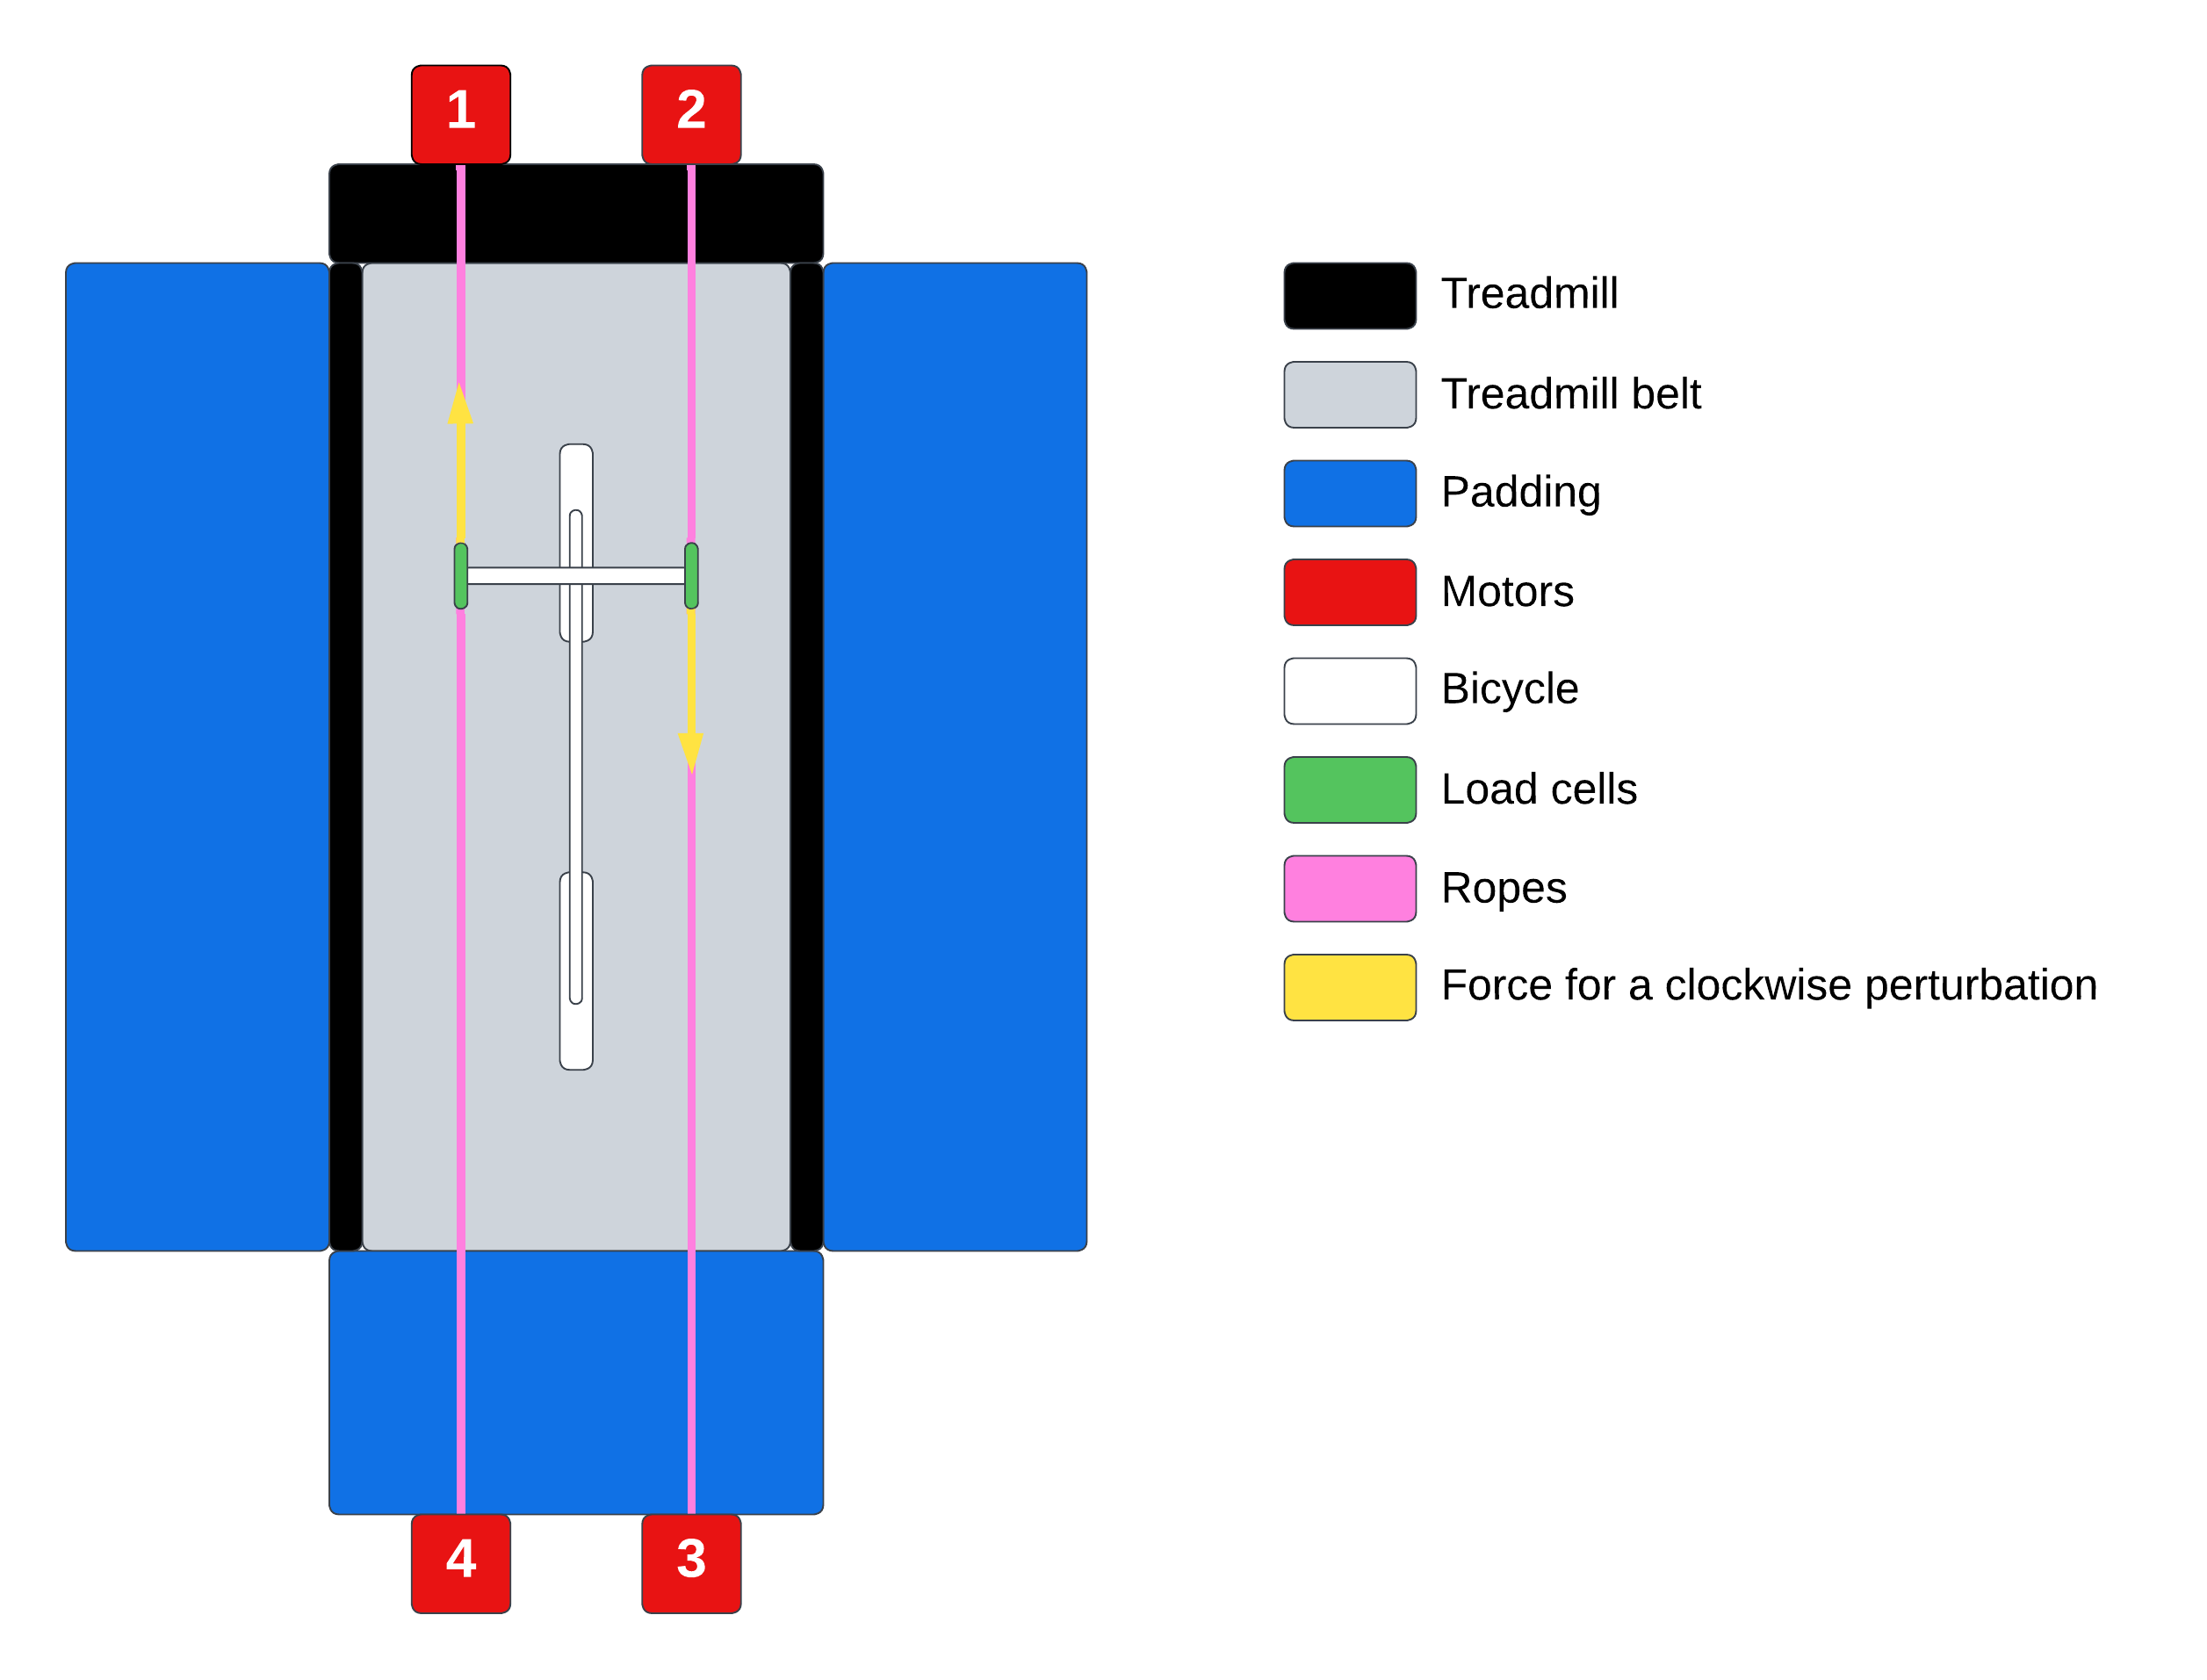
\includegraphics[height=65mm]{figures/setup-diagram.png}}
  \subcaptionbox{A participant on the bicycle in the safety harness with the
    Bump'Em motor lines attached to the ends of the
    handlebars.\protect\label{fig:participant-in-set-up}}
    {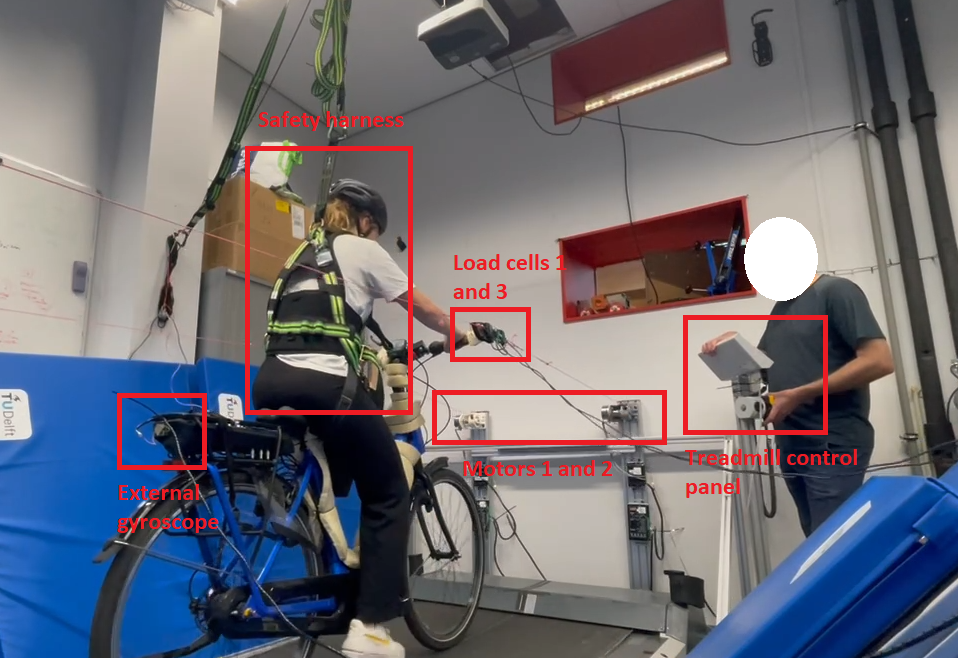
\includegraphics[height=65mm]{figures/participant-in-set-up.png}}
  \caption{Diagrams showing the Bump'Em system arranged to apply handlebar
    perturbations and the various system components.}
  \label{fig:experimental-setup}
\end{figure}

\subsection{Protocol}
%
We recruited 26 able-bodied young adults (20-36 years old) to participate in
the experiments. The participants were all confident in their cycling skills
and had cycled at least once in the last month. All participants consented to
the experiment and could decline to continue at any time. The study was
approved by Delft University of Technology's Human Research Ethics Council
(record \#3897).

The participants were divided into two groups. The first group of fifteen
participants performed the protocol at a belt speed of
10~\si{\kph}(2.8~\si{\mps}) with the controller gain value set to $g=8$ and the
second group of eleven particpants performed the protocol at a belt speed of
6~\si{\kph} (1.7~\si{\mps}) with the controller gain set to $g=10$. The
10~\si{\kph} group's experiments occurred two weeks before the 6~\si{\kph}
group.

Participants wore a helmet and they were attached to the ceiling via a fall
safety harness, Figure~\ref{fig:participant-in-set-up}. The harness allowed
free movement pre-fall. The participants practiced riding on the treadmill
until they indicated they were comfortable enough to have perturbations
applied. For most, this was less than a 10~\si{\minute} warm up. We then asked
the rider to ride for 90~\si{\second}, while attempting to maintain the
location of their front wheel on the center line of the treadmill as a baseline
measure before the perturbations. We then applied perturbations in random
directions (clockwise or counter-clockwise), starting at 20~\si{\newton} and
increasing the magnitude by 30~\si{\newton} until the participants fell. We
defined a ``fall'' on the treadmill by two criteria: 1) the rider removes their
foot from the pedal and places it on the ground or 2) the bicycle wheel exceeds
the width of the treadmill belt. Figure~\ref{fig:perturbation-sequence} shows
an example resulting motion from a perturbation. We logged the force magnitude
that caused the first fall to characterize that participant's
\emph{perturbation resistance threshold}.
%
\begin{figure}
  \centering
  \subcaptionbox{Before perturbation}{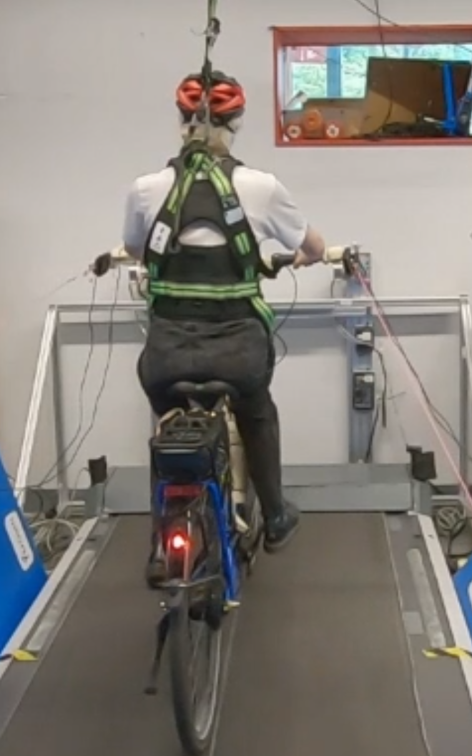
\includegraphics[width=60mm]{figures/start.png}}
  \subcaptionbox{During perturbation}{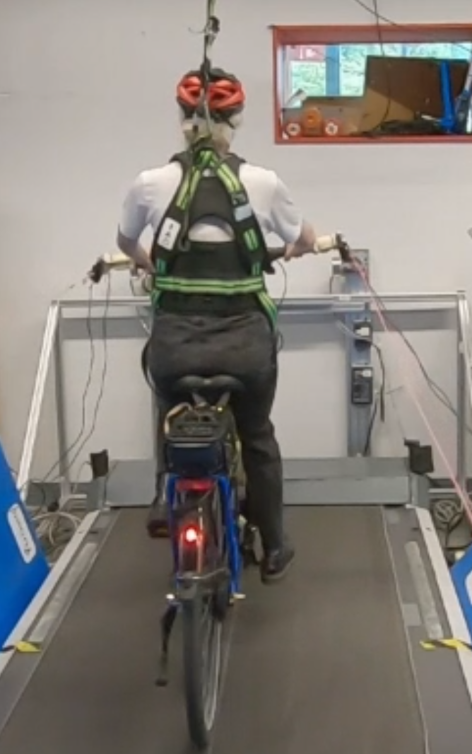
\includegraphics[width=60mm]{figures/during.png}}
  \subcaptionbox{After perturbation}{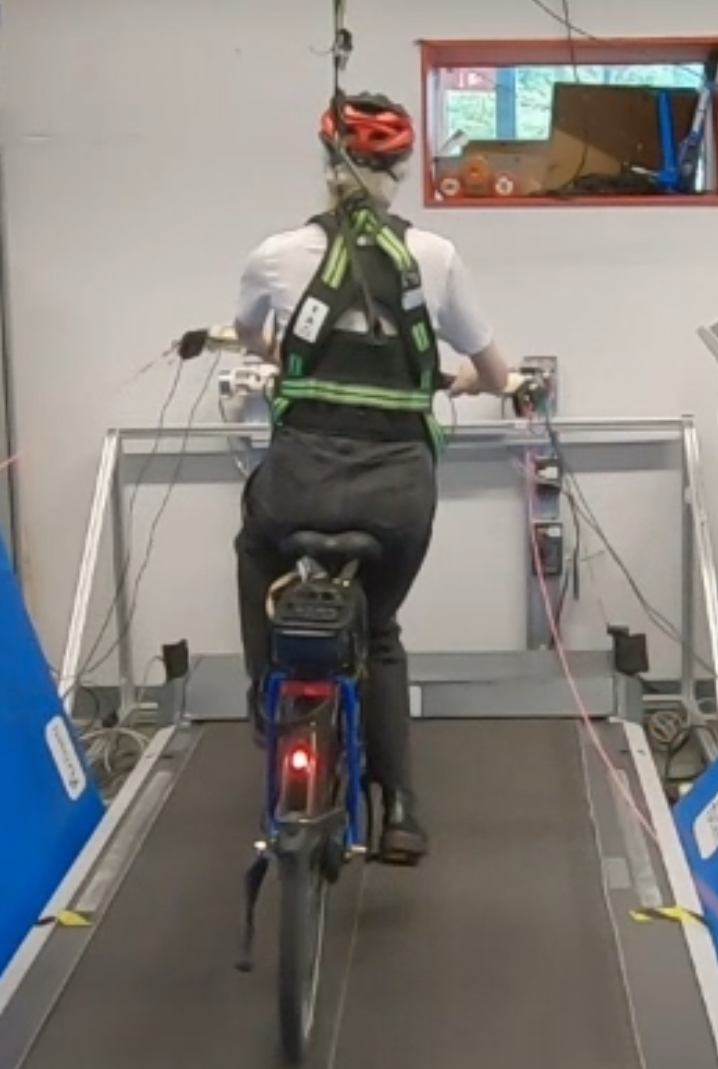
\includegraphics[width=60mm]{figures/after.png}}
  \subcaptionbox{Recovery from perturbation}{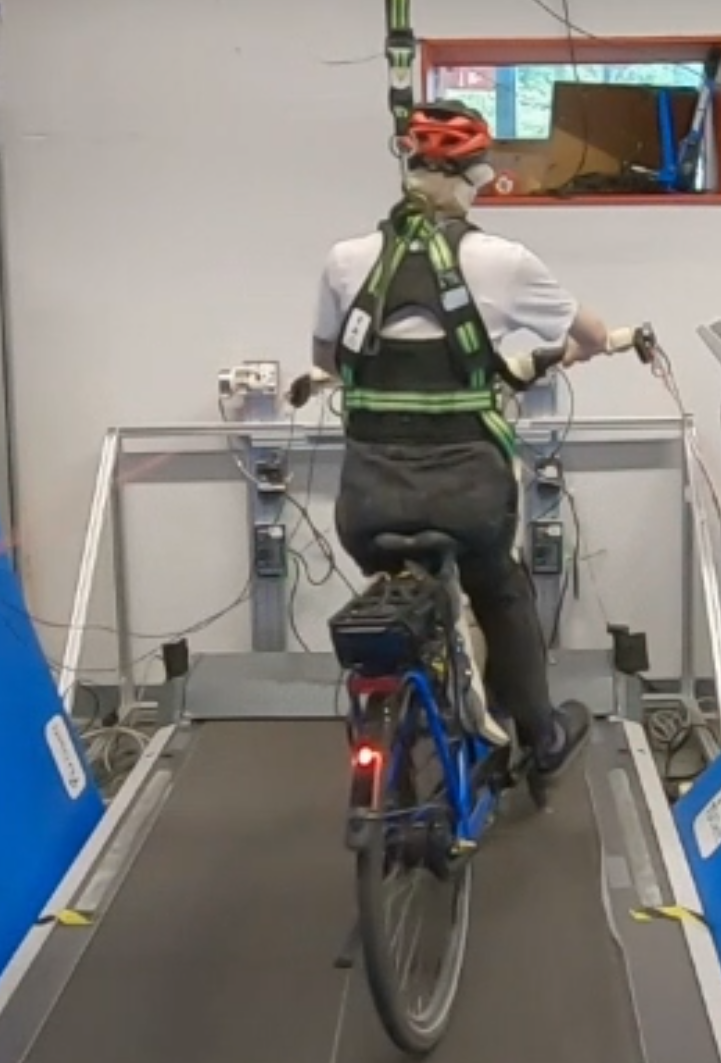
\includegraphics[width=60mm]{figures/recovery.png}}
  \caption{Video frames depicting the application of a perturbation and the
  rider's response and recovery.}
  \label{fig:perturbation-sequence}
\end{figure}

Following the initial threshold determination, we choose perturbation forces
according to a random and adaptive staircase procedure applying perturbations
above and below the initial perturbation threshold, while allowing small
progression of the perturbation threshold to accommodate learning effects. Five
possible perturbation forces are determined based on the initial perturbation
threshold estimate: the initial estimate itself, two perturbations lower than
the initial estimate, and two perturbations higher than the initial estimate.
The five possible perturbations are separated by 10~\si{\newton} steps. For
example, if the initial estimate of the perturbation threshold of a participant
is 80~\si{\newton}, the five possible perturbations are 60, 70, 80, 90 and
100~\si{\newton}. Which one of these five perturbations is chosen first is
determined at random. If the perturbation results in a fall, the estimate of
the perturbation threshold is decreased by 10~\si{\newton}, and vice versa if
the perturbation did not result in a fall. Five new possible perturbation
forces are determined around the updated perturbation threshold, and a new
perturbation is selected at random. This process iterates until twenty
perturbations are applied. The goal of this adaptive staircase procedure is to
have participants fall for approximately 50\% of the time. After the first set
of 20 perturbations, we let the cyclist rest and then perform another 20
perturbations. We randomize whether the balance assist system is on or off
during the first or second set of 20 perturbations for each participant.

\subsection{Measurements}
%
We measure the time histories of the Bump'Em delivered perturbation forces and
the bicycle's steer angle \(\delta\), roll angle \(\phi\), roll angular rate
\(\dot{\phi}\), and forward speed \(v\). Figure~\ref{fig:perturbation_0} shows
an example perturbation force measurement compared to our Bump'Em controller
command.
%
\begin{figure}
  \centering
  \includegraphics[width=140mm]{figures/torque_angle_perturbation_10.png}
  \caption{Externally applied perturbation torque alongside the resulting
    measured motion and steer motor induced torque based on a 110~\si{\newton}
    counterclockwise applied force at a 6~\si{\kph} travel speed. The circles
    on the roll and steer angle plot show the angles \(\phi_0\) and
    \(\delta_0\) at the perturbation start.}
  \label{fig:perturbation_0}
\end{figure}

Based on findings from measuring riders without balance assist in
\citet{Haitjema2023a}, we calculate several variables that we hypothesize may
influence fall probability. We use the angular impulse \(L\) of the
perturbation forces over a 0.3~\si{\second} duration to characterize the
magnitude of delivered perturbation. The duration is selected based on the
duration of the commanded force and is calculated as follows:
%
\begin{align}
  L =
  \int_{0\si{\second}}^{0.3\si{\second}} \frac{l}{2}(F_r + F_l) dt
  =
  \int_{0\si{\second}}^{0.3\si{\second}} \frac{l}{2}\left[(F_{rf} - F_{rr}) + (F_{lf}
  - F_{lr})\right] dt
  \textrm{.}
  \label{eq:angular-impulse}
\end{align}

where \(F_r\) and \(F_l\)  is the total force applied on the right and left
handlebar ends, respectively which are the sum of the rear and front load cell
readings \(F_{rr}\) and \(F_{rf}\), for example. The handlebar length is given
as \(l\) in Equation \ref{eq:angular-impulse}. We use angular impulse instead
of peak torque to normalize for the duration of the applied perturbation.

We record the order number of each perturbation \(j\), i.e. first, second,
third, \ldots, to measure how many perturbations a rider is subjected to before
the current perturbation. At the initiation of each perturbation we log the
instantaneous steer and roll angles to characterize the configuration of the
bicycle when perturbed. The gain setting on the balance assist controller
indicates if the assistance is off \(g=0\) or on at two different levels: low
\(g=8\) or high \(g=10\). A recovery from the perturbation is successful if the
person neither places their foot down onto the treadmill surface nor their
wheel of the bicycle exits the width of the treadmill belt. We record this as a
binary variable \(f\) for "fall". All measured variables are reported in
Table~\ref{tab:raw}.
%
\begin{table}
  \centering
  \caption{Raw measurements taken during each trial. ``Fall Outcome'' and
    ``Perturbation Order Number'' are recorded per perturbation instance. The
    remaining measures are time varying during each trial.}
  \begin{tabular}{llll}
    \toprule
    Measure & Variable & Units & Sensor \\
    \midrule
    Balance Assist Gain & \(g\) & \si{\newton\second\squared} & NA \\
    Bicycle Speed & \(v\) & \si{\meter\per\second} & wheel encoder \\
    Fall Outcome & \(f\) & boolean & NA \\
    Force \(l\)eft/\(r\)ight,\(f\)ront/\(r\)ear &
    \(F_{lf},F_{rf},F_{lr},F_{rr}\) & \si{\newton} & inline load cell\\
    Perturbation Order Number & \(j\) & integer & NA\\
    Roll Angle & \(\phi\) & \si{\degree} & BN0086 Kalman estimate \\
    Roll Angular Rate & \(\dot{\phi}\) & \si{\degree\per\second} & BN0086 rate gyroscope \\
    Steer Angle & \(\delta\) & \si{\degree} & steer tube encoder \\
    \bottomrule
  \end{tabular}
  \label{tab:raw}
\end{table}

\subsection{Statistics}
%
We test our hypothesis that the balance assist controller will reduce the
probability of falling when perturbed externally at the handlebar. We have a
single binary fall outcome variable \(f\) that is dependent on several possible
explanatory independent variables, one of which is the binary balance assist
state (on or off). See Table~\ref{tab:stat-model-variables} for the statistical
model variables.
%
\begin{table}
  \centering
  \caption{Independent and dependent variables used in the statistical
    regression model.}
  \label{tab:stat-model-variables}
  \begin{tabular}{llll}
    \toprule
    Variable & Causality & Units & Description \\
    \midrule
    \(L\)        & independent & \si{\newton\meter\second} & angular impulse of perturbation torque \\
    \(\delta_0\) & independent & \si{\degree} & steer angle at start of perturbation \\
    \(\phi_0\)   & independent & \si{\degree} & roll angle at start of perturbation \\
    \(f\)        & dependent   & boolean & outcome: did not fall 0 or did fall 1 \\
    \(c\)        & independent & boolean & balance assist: off 0 or on 1 \\
    \(j\)        & independent & integer & order number of perturbation \\
    \bottomrule
  \end{tabular}
\end{table}

Fall outcome \(f_{ij}\) is the binary outcome of perturbation \(j\) on
participant \(i\) which follows a Bernoulli distribution given the probability
\(p_{ij}\) that a fall occurs:
%
\begin{align}
  f_{ij} | p_{ij} \sim \textrm{Bernoulli}(p_{ij}) \textrm{.}
\end{align}
%
We evaluate our hypothesis using a multivariate logistic regression model that
represents the probability of this binary outcome. The log-odds of the
probability is then a linear function of our independent variables with
\(\beta\) being the intercept and \(\alpha_k\) the linear coefficients to the
\(K\) independent variables \(x_{ij}^k\), i.e. all variables in
Table~\ref{tab:stat-model-variables} except \(f\).
%
\begin{align}
  \log \left(\frac{p_{ij}}{1-p_{ij}} \right) =
  \beta + \sum_{k=0}^{K} \alpha_k x_{ij}^{k}
  \label{eq:log-regress}
\end{align}

Before fitting the model, we scale each independent variable \(x_{ij}^k\) such
that they have a mean of zero and a standard deviation of one by cluster-mean
centering, as recommended by \citet{Enders2007}, with clusters being an
individual participant. The clusters are chosen as all data from an individual
participant because we are only interested in the association between the state
of the balance assist system and the outcome of the perturbation. We expected
there to be a variation between participants in how well they are able to
resist the perturbation. However, this was not true. Cluster-mean centering
showed there to be no variation between participants. This fact allows us to
utilize a simple single-level logistic regression model, instead of a
multilevel model. This left us with angular impulse, perturbation order,
balance assist state, and roll \& steer angles at the time of perturbation as
independent variables. We also include interaction effects between the balance
assist state and the other four variables. We divide the analysis into two
separate model evaluations, one for the 6~\si{\kph}, \(g=10\) trials and one
for the 10~\si{\kph}, \(g=8\) trials and we evaluate our hypothesis for each
set of data. Statistics were computed with the lme4 version
1.1~\citep{Bates2015} package in R version 4.1.3~\citep{RCoreTeam2021}.

\section{Results}
%
The coefficient estimates for a single-level logistic regression for the data
from the 6~\si{\kph}, gain $g=10$ trials are shown in
Table~\ref{tab:freq-coefs-6}. The angular impulse, perturbation order, and
balance assist state are all statistically significant predictors with angular
impulse having a dominant effect. Larger angular impulse increases the
probability to fall and both enduring more perturbations or having the balance
assist on, decrease the probability to fall. The associated multiplicative
change in odds are shown in Table~\ref{tab:freq-coefs-6}.
%
\begin{table}
  \centering
  \caption{Logistic regression coefficient estimates \(\alpha_k\) at
    6~\si{\kph} and gain $g=10$ along with the standard error SE, p-value
    \(p\), multiplicative change in odds \(e^{\alpha_k}\), and the 5\%
    confidence interval bounds.}
  \label{tab:freq-coefs-6}
  \begin{tabular}{lrrrrrr}
    \toprule
    Variable & \(\alpha_k\) & SE & \(p\) & \(e^{\alpha_k}\) & 2.5\% & 97.5\% \\
    \midrule
    Intercept \(\beta\)                           & -0.29 & 0.17 & 0.09 & 0.75 & 0.53 & 1.05 \\
    Angular impulse \(L\)                         & 1.69 & 0.27 & 0.00\(^*\) & 5.40 & 3.18 & 9.16 \\
    Perturbation order \(j\)                      & -0.77 & 0.22 & 0.00\(^*\) & 0.46 & 0.30 & 0.72 \\
    Balance assist state \(c\)                    & -0.64 & 0.27 & 0.02\(^*\) & 0.53 & 0.31 & 0.89 \\
    Roll angle \(\phi_0\)                         & -0.25 & 0.21 & 0.24 & 0.78 & 0.51 & 1.18 \\
    Steer angle \(\delta_0\)                      & -0.14 & 0.21 & 0.51 & 0.87 & 0.58 & 1.32 \\
    Balance assist state $\times$ roll angle         & 0.52 & 0.34 & 0.12 & 1.68 & 0.86 & 3.29 \\
    Balance assist state $\times$ steer angle        & -0.41 & 0.34 & 0.22 & 0.66 & 0.34 & 1.28 \\
    Balance assist state $\times$ angular impulse    & 0.41 & 0.41 & 0.32 & 1.51 & 0.67 & 3.38 \\
    Balance assist state $\times$ perturbation order & -0.53 & 0.34 & 0.12 & 0.59 & 0.30 & 1.15 \\
    \bottomrule
  \end{tabular}
\end{table}

The coefficient estimates for a single-level logistic regression at
10~\si{\kph} with gain $g=8$ are shown in Table \ref{tab:freq-coefs-10}. The
angular impulse and perturbation order are statistically significant predictors
with angular impulse being the dominant effect. Larger angular impulse
increases the probability to fall and enduring more perturbations decreases the
probability to fall. Unlike the 6~\si{\kph} trials, the balance assist state is
not a significant predictor but the effect would be a reduction in the
probability to fall if it were. At both speeds, the angular impulse has about
twice the magnitude in effect as the perturbation order.
%
\begin{table}
  \centering
  \caption{Logistic regression coefficient estimates \(\alpha_k\) at
    10~\si{\kph} and gain $g=8$ along with the standard error SE, p-value
    \(p\), multiplicative change in odds \(e^{\alpha_k}\), and the 5\%
    confidence interval bounds.}
  \label{tab:freq-coefs-10}
  \begin{tabular}{lrrrrrr}
    \toprule
    Variable & \(\alpha_k\) & SE & \(p\) & \(e^{\alpha_k}\) & 2.5\% & 97.5\% \\
    \midrule
    Intercept                & -0.24 & 0.16 & 0.13 & 0.78 & 0.57 & 1.07 \\
    Angular impulse \(L\)    & 2.39  & 0.29 & 0.00\(^*\) & 10.92 & 6.23 & 19.13 \\
    Perturbation order \(j\) & -1.16 & 0.21 & 0.00\(^*\)  & 0.31 & 0.21 & 0.48 \\
    Balance assist on \(c\)  & -0.44 & 0.24 & 0.07 & 0.64 & 0.40 & 1.03 \\
    Roll angle \(\phi_0\)    & 0.27  & 0.22 & 0.22 & 1.31 & 0.85 & 2.04 \\
    Steer angle \(\delta_0\) & -0.37 & 0.24 & 0.12 & 0.69 & 0.43 & 1.10 \\
    Balance assist state $\times$ roll angle         & -0.61 & 0.34 & 0.08 & 0.54 & 0.28 & 1.07 \\
    Balance assist state $\times$ steer angle        & 0.56  & 0.35 & 0.11 & 1.76 & 0.88 & 3.50 \\
    Balance assist state $\times$ angular impulse    & 0.46  & 0.44 & 0.29 & 1.59 & 0.68 & 3.74 \\
    Balance assist state $\times$ perturbation order & -0.37 & 0.32 & 0.25 & 0.69 & 0.37 & 1.30 \\
    \bottomrule
  \end{tabular}
\end{table}

Turning the balance assist system on significantly \((p<0.05)\) reduces the
odds that a perturbation results in a fall while cycling at a speed of
6~\si{\kph}. Figure~\ref{fig:probability-6kph} visualizes the probability of
falling as a function of the mean and centered angular impulse per participant
for the balance assist state on and off while keeping all other explanatory
factors at their centered mean values. This figure is created by setting all
explanatory variables to their mean and calculating the probability from
Equation~\ref{eq:log-regress} for only change in angular impulse given the
estimates in Table~\ref{tab:freq-coefs-6}. The table indicates that the balance
assist system halves (0.53) the odds that a perturbation results in a fall.
This figure shows that for relatively large impulses the probability to fall is
unity for both states of balance assist on and off. And for relatively small
impulses the probability to fall is null for both states. But for impulses in
the magnitude region (about -1 to 0.5 STD), i.e. around the mean-centered
perturbation resistance threshold, the probability of falling is significantly
lowered with the balance assist system on. The skewness of the probability
curves arrives from the interaction effects. Figure~\ref{fig:probability-10kph}
shows the same result for the 10~\si{\kph} trials which has a similar trend of
reducing the probability to fall with the balance assist system turned on, but
the effect is not significant.
%
\begin{figure}
  \centering
  \subcaptionbox{Fall probability for the 6~\si{\kph} trials.
    \label{fig:probability-6kph}}{
    \includegraphics[width=80mm]{figures/predicted_fall_probability_6kmh.png}
  }
  \subcaptionbox{Fall probability for the 10~\si{\kph} trials.
    \label{fig:probability-10kph}}{
    \includegraphics[width=80mm]{figures/predicted_fall_probability_10kmh.png}
  }
  \caption{Comparison of predicted fall probability for balance assist on
    (solid) or off (dashed) when all other predictor variables are fixed at zero,
    except for the interaction effect between the balance assist and the
    angular impulse. The abscissa is the standard deviation around the mean
    (all perturbations), centered per participant.}
  \label{fig:probability}
\end{figure}

\section{Discussion}
%
We have shown that at a 6~\si{\kph} riding speed the addition of balance assist
control reduces the chance that a rider will fall when perturbed around the
limits of their control authority. But this effect diminishes just below
significance at the higher speed scenario of 10~\si{\kph}. We were only able to
test these two speed-gain scenarios for mostly homogeneous sets of riders
within the resources of this research project, but additional experimental work
could help understand more completely the range and limits of the positive
effect of the balance system. For example, it is possible that simply
increasing the controller gain at 10~\si{\kph} also results in a significant
positive effect. A longitudinal study of normal use of the balance assist
bicycle compared to a control group could provide the strongest evidence of any
benefit we have seen in this specific scenario.

\subsection{Stability and Human Controlled Plant Dynamics}
%
The linear Carvallo-Whipple model indicates that the steer controller
stabilizes the bicycle-rider system, but this model assumes the rider's hands
are not connected to the handlebars and that they clamp their body as rigidly
as possible to the rear frame. In reality, the system's behavior is likely more
akin to a marginally stable or an easily controllable unstable system due to
the various un-modeled effects. Our system may not result in a definitely
stable system, i.e. cannot fall, but having plant eigenvalues with very small
unstable eigenvalue real parts correlates to ease of control~\citep{Hess2012}.

The controller design we utilize, Equation~\ref{eq:implemented-controller},
also increases the weave mode frequency by a factor of about three up in a
bandwidth of about 1~\si{\hertz}. This bandwidth is still controllable by the
human's neuromuscular system, but may feel unusual as it is more akin to what
the steering would feel like at in the \SIrange{30}{40}{\kph} speed range.
\Citet{Hanakam2023} reported dissatisfaction in subjective rider feeling on
their similar bicycle to ours and this effect to the human-controlled plant
dynamics could be an explanation to their findings.

\subsection{Utility of the Logistic Model and Extrapolation to Natural Falls}
%
The probability that a fall occurs depends on the values of all the independent
variables in Table~\ref{tab:stat-model-variables}, but we can visualize the
effect of one or two variables (e.g. Figure~\ref{fig:probability}) to gain some
insight.
To interpret the results in Tables~\ref{tab:freq-coefs-6} and
\ref{tab:freq-coefs-10} it is important to understand the relationship between
probability and odds.
The estimate in Table~\ref{tab:freq-coefs-6} shows that the balance assist
system halves the odds that a perturbation results in a fall:
\(e^{\alpha_k}=0.53\).
This means if the odds are a 1000:1, turning on the balance assist system
reduces the odds to 500:1.
However, in that case the probability that a fall occurs is only reduced from
$0.999$ to $0.998$.
If the odds that a fall occurs are smaller, halving the odds has a larger
influence on the fall probability.
For example, if the odds that a fall occurs is two, halving it to one reduces
the probability from $0.66$ to $0.50$.
This can be seen in Figure~\ref{fig:probability} which shows the fall
probability as a function of the magnitude of the normalized angular impulse
for both speeds.
The difference in probability between the balance assist on/off case becomes
insignificant outside of approximately \(\pm1\) standard deviation of the
average angular impulse the rider was subjected to.
This means that the balance assist is most effective for perturbations close to
the participant's perturbation resistance threshold and that large
perturbations will make you fall regardless of the balance assist's help.

To illustrate the effect of the balance assist system on fall probability, we
will give an example of how the data collected during the experiments is used
to predict fall probability. We use Equation~\ref{eq:log-regress} and the
coefficients in Table~\ref{tab:freq-coefs-6}. For simplicity's sake, the
interaction effects are not included. For example, assuming that the mean
angular impulse $\bar{L}$ of all the perturbations applied to a participant is
100~\si{\newton} and the standard deviation $\sigma_{L}=15$. The centered and
scaled angular impulse can be calculated by subtracting $\bar{L}$ from the
applied angular impulse $L$, and dividing this by $\sigma_{L}$. The same
applies for the perturbation order $j$, initial roll angle $\phi_0$, and
initial steer angle $\delta_0$. If we take the coefficients estimated for
cycling at 6~\si{\kph}, the log-odds of falling can be calculated as follows.
\todo{Check this equation, where is \(\bar{L}\) 100N in the equation?}
%
\begin{equation}
  \begin{split}
    \log \left( \frac{p_{ij}}{1-p_{ij}} \right)
    = & \quad
    \beta + \sum_{k=1}^{k=5}\alpha_k \frac{x_{ij}^{k}-\bar{x}_{ij}^{k}}{\sigma^{x^{k}}} \\
    = &
   -0.29 + 1.69\cdot\frac{110~\si{\newton} - 115\si{\newton}}{15\si{\newton}} -0.77\cdot\frac{10-20}{11.54}  \\
    & -0.25\cdot\frac{-6\si{\degree}-2\si{\degree}}{10\si{\degree}}
    -0.14\cdot\frac{1\si{\degree}+3\si{\degree}}{5\si{\degree}} -0.64\cdot c \\
    = &
    1.42 -0.64 \cdot c
  \end{split}
\end{equation}
%
The state of the balance assist \(c\) is a binary variable. If the
balance assist is turned on, the log-odds that a fall occurs are decreased by
0.64. The odds and probability can be calculated:
%
\begin{align}
  \frac{p_{ij}}{1-p_{ij}} & = e^{1.42-0.64c} = e^{1.42}\cdot e^{-0.64s} = 4.14 \cdot 0.53c \\
  p_{ij}|_{c=0} & = \frac{4.14}{1 + 4.14} = 0.81 \\
  p_{ij}|_{c=1} & = \frac{4.14\cdot0.53}{1 + 4.14\cdot{0.53}} = 0.69
\end{align}
%
Turning on the balance assist system reduces the probability that the
perturbation results in a fall from 81\% to 69\% in this case.

This illustration alludes to the difficulty needed to apply the model in way
that could predict how many falls may be averted in a natural setting if the
balance assist system is used. Estimates of the predictor variables extracted
from the limited data collected from natural cycling would be needed to
populate the model.

The positive effect of the balance assist system is coupled to the assumptions
and experimental scenarios we implemented and there is unfortunately no simple
way to extrapolate our results to reductions of single-actor crashes we may see
if such a system were deployed widely to bicyclists. Although, our results do
indicate that we would see such a reduction, even if only in a class of
single-actor crashes that most resemble our experimental design. If there were
more comprehensive and detailed natural data of how people fall we could make
estimates on the number of falls reduced if everyone road a balance assist
bicycle.

\subsection{Treadmill Width}
%
Angular impulse magnitude has the largest significant effect for predicting
fall probability as seen in both Tables~\ref{tab:freq-coefs-6} and
\ref{tab:freq-coefs-10}. An increase in angular impulse increases the fall
probability both at 6 and 10~\si{\kph}. At 10~\si{\kph}, the multiplicative
change in odds is approximately twice as big as at 6~\si{\kph}. Thus, angular
impulse is a more important predictor at higher speeds compared to lower
speeds. We posit that this likely has to do with the width of the treadmill and
that this could also be why the balance assist system did not have a
statistically significant effect at 10~\si{\kph}. As a bicycle travels at
higher speeds, the same perturbation magnitude causes larger lateral
deviations. At 10~\si{\kph} almost all falls were due to the bicycle exiting
the maximum width of the treadmill. If the same experiment was performed on an
infinitely wide plane, the riders may have recovered from more perturbations.
At 6~\si{\kph} the riders could often recover in the allotted treadmill width
due to the smaller lateral deviations. We believe our results are very much
dependent on the two modes of falling, i.e. exit the treadmill width or foot is
placed on the belt. On the other hand, Cycle paths are a similar width as the
treadmill, so rider's are often limited in width when recovering from a fall
thus exiting the treadmill width may be an appropriate measure for indicating a
fall.

\subsection{Learning Effect}
%
An increase in the number of perturbations that a participant already
experienced, decreases the probability that a fall occurs. This is likely due
to the participants learning how to better recover from the perturbation over
the duration of the experiment. This effect is significant at both 6 and
10~\si{\kph}, and in the same order of magnitude. This suggests that the
learning effect that occurs during the experiment is not strongly dependent on
the speed.

\subsection{Non-significant Predictors}

Roll and steer angle at the initiation of a perturbation are not a significant
predictor of fall probability at 6 or at 10~\si{\kph}. We expected these
variables to have a significant effect based on the following reasoning. If you
are in a rolled and steered state that is far from the upright equilibrium,
then a perturbation that further pushes you from the equilibrium should have
some additive or multiplicative effect on the resulting motion trajectory and
make it harder to recover from a fall.

None of the interaction effects are statistically significant. That means that
whether the balance assist system is on or off does not significantly change
the effect that the roll angle, steer angle, angular impulse, and perturbation
order have on the probability that a fall will occur.

\section{Conclusion}
%
Automatically controlling a steering motor in a bicycle using roll rate
feedback lowers the speed at which the bicycle is stable. This makes the
bicycle's low speed dynamics more akin to its uncontrolled high speed dynamics,
which is easier for a rider to control in balance. Perturbation forces applied
to the handlebar can cause a rider to fall and every rider has a perturbation
magnitude threshold at which they are more likely to fall than not. The
probability of falling when mechanically perturbed is significantly reduced
when traveling at 6~\si{\kph} when the balance assisting control is activated.
This effect is present when traveling at 10~\si{\kph} but more investigation is
needed to determine if the effect can be significant. The positive effect to
balance is rider independent and most effective in the regime of perturbations
near the limits of the rider's control authority. Given that similar effects
cause falls during bicycling, use of the balance assist system in real world
use cases will reduce the number of falls at low bicycling speeds.

\section*{Acknowledgements}
%
This study follows and draws from experimental and analysis methods originally
developed in unpublished research by Marco Reijne. The authors acknowledge
Felix Dauer, David Gabriel, Sierd Heida, Oliver Maier, Maarten Pelgrim, Marco
Reijne, and Arend Schwab for contributions to the development of the balance
assist bicycle. We acknowledge Shannon van de Velde and Marco Reijne's
development of the bicycle perturbation system. Allen Downey provided useful
insight in the statistical condsiderations. We thank all of the assistants that
helped run the experiments and the participants for their time an enthusiasm.
We thank Peter Stahlecker for valuable feedback in early revisions.

\section*{Funding}
%
This study is funded by Dutch Research Council, Nederlandse Organisatie voor
Wetenschappelijk Onderzoek (NWO), under the Citius Altius Sanius program and in
collaboration with Bosch eBike Systems and Royal Dutch Gazelle. The funders had
no role in the data collection and analysis or preparation of the manuscript.

\section*{Code and Data Availability}
%
The data and code to reproduce the paper are available at:

\noindent
\url{https://github.com/mechmotum/fall-probability-paper}

\printbibliography

\appendix
%
\section{Physical Parameters}
\label{sec:physical-parameters}
%
Physical parameters and estimated uncertainties (standard deviation) for the
balance assist bicycle with and without a rider. These are found using the
measurement approach for geometric and inertial parameters for a bicycle
explained in \citet{Moore2012}. The rider inertial parameters are derived from
the 83.5~\si{\kilogram} rider ``Jason'' available in BicycleParameters
1.1.1~\citep{Moore2024}. The variable names match the notation and definitions
from the benchmark bicycle model presented in
\citet{Meijaard2007}.\todo{Uncertainties are based on best guess for
uncertainty in the raw measurements, may be better to remove them as they
aren't so meaningful.}
%
\begin{table}[h]  % have to use "h" so that it stays within the appendix
  \centering
  \caption{Physical parameters of the balance assist bicycle with and without
    the inertia effects of a rigid rider.}
  \begin{tabular}{llrrrr}
    \toprule
    Variable & Unit & Without Rider & Uncertainty & With Rider & Uncertainty \\
    \midrule
    \(c\) & \si{\meter} & 0.04 & 0.01 & 0.04 & 0.01 \\
    \(g\) & \si{\meter\per\second\squared} & 9.80665 & NA & 9.80665 & NA \\
    \(I_{Bxx}\) & \si{\kilogram\meter\squared} & 1.12 & 0.02 & 19.7 & 0.3 \\
    \(I_{Bxz}\) & \si{\kilogram\meter\squared} & 0.05 & 0.03 & -3.5 & 0.2 \\
    \(I_{Byy}\) & \si{\kilogram\meter\squared} & 3.16 & 0.08 & 22.7 & 0.4 \\
    \(I_{Bzz}\) & \si{\kilogram\meter\squared} & 2.12 & 0.03 & 5.0 & 0.1 \\
    \(I_{Fxx}\) & \si{\kilogram\meter\squared} & 0.0995 & 0.0005 & 0.0995 & 0.0005 \\
    \(I_{Fyy}\) & \si{\kilogram\meter\squared} & 0.1902 & 0.0009 & 0.1902 & 0.0009 \\
    \(I_{Hxx}\) & \si{\kilogram\meter\squared} & 0.298 & 0.003 & 0.298 & 0.003 \\
    \(I_{Hxz}\) & \si{\kilogram\meter\squared} & -0.038 & 0.007 & -0.038 & 0.007 \\
    \(I_{Hyy}\) & \si{\kilogram\meter\squared} & 0.257 & 0.006 & 0.257 & 0.006 \\
    \(I_{Hzz}\) & \si{\kilogram\meter\squared} & 0.057 & 0.003 & 0.057 & 0.003 \\
    \(I_{Rxx}\) & \si{\kilogram\meter\squared} & 0.1023 & 0.0006 & 0.1023 & 0.0006 \\
    \(I_{Ryy}\) & \si{\kilogram\meter\squared}& 0.1887 & 0.0007 & 0.1887 & 0.0007 \\
    \(\lambda\) & \si{\radian} & 0.25 & 0.03 & 0.25 & 0.03 \\
    \(m_B\) & \si{\kilogram} & 22.50 & 0.01 & 106.00 & 0.01 \\
    \(m_F\) & \si{\kilogram} & 2.23 & 0.01 & 2.23 & 0.01 \\
    \(m_H\) & \si{\kilogram} & 4.30 & 0.01 & 4.30 & 0.01 \\
    \(m_R\) & \si{\kilogram} & 4.08 & 0.01 & 4.08 & 0.01 \\
    \(r_F\) & \si{\meter} & 0.3523 & 0.0001 & 0.3523 & 0.0001 \\
    \(r_R\) & \si{\meter} & 0.3489 & 0.0001 & 0.3489 & 0.0001 \\
    \(w\) & \si{\meter} & 1.113 & 0.008 & 1.113 & 0.008 \\
    \(x_B\) & \si{\meter} & 0.52 & 0.01 & 0.374 & 0.002 \\
    \(x_H\) & \si{\meter} & 0.92 & 0.02 & 0.92 & 0.02 \\
    \(z_B\) & \si{\meter} & -0.52 & 0.02 & -1.009 & 0.003 \\
    \(z_H\) & \si{\meter} & -0.860 & 0.006 & -0.860 & 0.006 \\
    \bottomrule
  \end{tabular}
\end{table}

\end{document}
